\section{Forward and backward propagation}

  There are two main differences between the forward and backward pass
  computation.  While the forward pass computes convolutions, the
  backward pass computes cross--correlations.  Performing a
  cross--correlation is equivalent to performing a convolution with
  kernel that is reflected along all dimensions.  Secondly, during the
  forward pass the convolution is performed only for locations where
  the kernel is fully contained inside the image\footnote{This is
    known as a \texttt{valid} convolution in MATLAB.}.  Thus, the
  output image has dimensions smaller or equal to the input image.  In
  the backward pass, \texttt{full} convolution/cross--correlation is
  performed.  Image size increases because an output voxel exists
  whenever the sliding window has some overlap with the input image.

  Given an algorithm for the forward pass, a backward pass can be
  implemented by (1) reflecting the kernels along all directions, thus
  converting cross--correlation to convolution, and (2) zero--padding
  the input image such that \texttt{valid} convolution becomes
  \texttt{full} convolution.

  We propose an algorithm for the forward pass that can handle an
  arbitrary zero padding of input image, thus the same algorithm can
  be used for the backward pass.  We assume that two copies of kernels
  are stored - original and reflected.  Both sets of kernels will be
  updated during the update phase.  This is reasonable because the
  memory required for kernels is typically much smaller than the
  memory required for the images.  Updating both sets of kernels
  instead of just one introduces very little overhead for the update
  phase, while allowing the reuse of the same algorithm for both the
  forward and backward computation.

  We will refer to the algorithm as the fwd-bwd algorithm.  Also,
  we'll refer to both the input/output images of the forward pass and
  the input/output gradients of the backward pass as
  \emph{input/output images}.  For simplicity, we will describe the
  details of the algorithm for the special case of 3D images.  Higher
  dimensions require adding an additional for loop in all of our
  primitives.

  \subsection{Algorithm overview}

  The result the computation of the fwd-bwd algorithm is $B$ sets of
  $F$ (or $F'$) $N$--dimensional images that can be represented as a
  $N+2$ dimensional tensor.  Computing the value of each element of
  the tensor is independent.  We assume that both $F$ and $F'$ are
  divisible by $S$, where $S$ is the width of the vector register.  On
  AVX2 enabled CPUs, $S$ is 8, and on AVX512, $S$ equals to 16.  This
  is reasonable as all state of the art networks for both registration
  and segmentation have both $F$ and $F'$ being a large multiple of
  $2$~\cite{krizhevsky2012imagenet, ronneberger2015u,
    simonyan2014very, sermanet2013overfeat, long2015fully,
    tran2015learning, ji20133d, maturana_iros_2015,
    maturana_icra_2014}.  An arbitrary number of images is supported
  by simply adding zero--initialized dummy images.  As both $F$ and
  $F'$ are relatively large, this would not introduce much
  computational overhead.  In further notation we will have $F =
  \alpha S$ and $F' = \alpha' S$.

  Our algorithm consists of a stack primitives with increasing
  complexity.  Each more complex primitives uses the less complex ones
  to perform more complex computation.  Before describing the details
  of each primitive, we list the primitives in the increasing order of
  complexity toghether with main motivation and goal for each one.

  \begin{enumerate}
  \item {\bf Sub--image primitive} -- a primitive that computes $S^2$
    convolutions on $S$ small images producing $S$ small images of
    size $R_D, R_H, R_W$.  The goal of this primitive is to
    efficiently re--use data in the register file as well as data in
    L1 cache.  The techinque used by the primitive is known as
    register blocking.
  \item {\bf Full image primitive} -- a primitive that computes $S^2$
    convolutions on $S$ images of an arbitrary size, producing $S$
    output images.  The primitives optimally divides the computation
    into small blocks for which the previous primitive is used.  The
    division and order of computation is designed for efficient use of
    hardware pre--fetching.
  \item {\bf Sub--layer primitive} -- a primitive that computes
    $\beta S$ images by performing $\alpha \beta S^2$
    convolutions on $\alpha S$ images.  The primitive is designed to
    efficiently utilize higher levels of cache (L2, L3).
  \item {\bf Full layer primitive} -- a static scheduler that divides
    the computation into above primitives and assigns each available
    core one or more such primitives.  The goal is to evenly divide
    the computation among available cores.
  \end{enumerate}

  We proceed to describe each primitive in details.

  \begin{algorithm}
    {\footnotesize
      \begin{codebox}
        \Procname{$\proc{Fwd-Bwd-Subtask} \langle \Theta, R_D, R_H, R_W, W_D, W_H, W_W \rangle(i,w,o,\theta)$}
        \li \kw{simd register} $oreg[R_D][R_H][R_W]$
        \li \kw{simd register} $wreg$
        \li \If $\Theta$ \Comment Static if
        \li \Then $oreg[:][:][:][:] \gets \theta$ \Comment Load bias
        \li \Else
        \li       $oreg[:][:][:][:] \gets \proc{LOAD}(o[:][:][:][:])$
        \End \li \kw{end if}
        \li \kw{for} $k_d \gets 0 \To W_D-1$
        \li   \Do \kw{for} $k_h \gets 0 \To W_H-1$
        \li      \Do \kw{for} $k_w \gets 0 \To W_W-1$
        \li         \Do \kw{for} $s \gets 0 \To S - 1$ \Comment Partially unrolled
        \li         \Do $wreg \gets w[k_d][k_h][k_w][s][:]$
        \li \kw{for} $d \gets 0 \To R_D-1$ \Comment Fully unrolled
        \li   \Do \kw{for} $h \gets 0 \To R_H-1$ \Comment Fully unrolled
        \li      \Do \kw{for} $w \gets 0 \To R_W-1$ \Comment Fully unrolled
        \li         \Do $oreg[d][h][w] \gets \proc{FMADD}($
        \li   \Do $wreg,$
        \li       $\proc{EXLOAD}(i[d+k_d][h+k_h][w+k_w][s]),$
        \li       $oreg[d][h][w][f])$
        \End \li \kw{end for} $w$
        \End \li \kw{end for} $h$
        \End \li \kw{end for} $d$
        \End \li \kw{end for} $s$
        \End \li \kw{end for} $k_w$
        \End \li \kw{end for} $k_h$
        \End \li \kw{end for} $k_d$
        \li $o[:][:][:][:] \gets \proc{STORE}(oreg[:][:][:][:])$
      \end{codebox}
    \caption{The finest granularity primitive that computes a
      sub--image of size $R_D \times R_H \times R_W$ of $S$ images by
      performing $S^2$ convolutions on $S$ input images with a kernel
      of size $W_D \times W_H \times W_W$.}
    \label{alg:serial-forward-subtask}
    }
  \end{algorithm}

  {\bf Sub--image primitive} \quad The lowest level primitive is shown
  in Algorithm~\ref{alg:serial-forward-subtask}.  The arguments inside
  the angled brackets are known during compile--time, while the
  arguments inside the parenthesis are provided during run--time.
  This means that the same function with different compile--time
  arguments will be separately compiled and optimized by the compiler.
  This is easily implemented using C++ templates.  Depending on the
  argument $\Theta$, the result of the convolution will be either
  accumulated to a given image, or the provided bias $\theta$ will be
  added to the result.

  In order for variables $oreg$ and $wreg$ to be stored in the
  register file, we need $R_D \times R_H \times R_W + 1$ to be smaller
  or equal to the number of available registers.  In C++ we have now
  way of explicitly telling the compiler to use registers, but instead
  we use regular vector variables (\texttt{\_\_m256} and
  \texttt{\_\_m512}) rather expect the compiler to automatically
  generate code that uses the register file.  As there are no more
  vector variables used in the function, this is an easy job for the
  compiler.  In lines 16--18, all values inside one vector register
  are multiplied by a scalar value and accumulated to another vector
  register (The procedure $\proc{EXLOAD}$ loads a scalar value to all
  $S$ locations in the vector register).  On AVX512 this two
  operations can be achieved by a single FMA instruction, while on
  AVX2 CPU, the scalar value has to be loaded into an auxiliary
  register before performing the fused multiply--add.  As AVX512 CPUs
  have $32$ vector registers, this limits $R_D \times R_H \times R_W$
  to $31$.  On the other side, due to need for auxiliary registers, on
  AVX2 CPUs the product is limited to $7$.  This is because we need
  $7$ extra auxiliary registers, plus one or storing $wreg$ while
  having $16$ available registers.

  The innermost loop over $S$ ensures efficient reuse of $L1$ cache.
  This is because the first pass through the loop will ensure that all
  cache--lines containing all elements for subsequent loops are in L1
  cache.  Most of these values will already be in $L1$ from the
  previous iterations of the outermost three loops.  Specifically,
  total of $(R_D+W_D-1) \times (R_H+W_D-1) \times (R_W+W_W-1)$ vector
  values have to be fetched to $L1$, which used exactly $S \times R_D
  \times R_H \times R_W \times W_D \times W_H \times W_W$ times.  The
  cache hit rate increases as the sizes of both the image and the
  kernel increase.  The cache miss rate can be thus approximated to
  $\frac{1}{S \times W_D \times W_H \times W_W}$.  Which is very low
  for even tiny kernels.  Cache misses are further reduced by hardware
  pre--fetching.

  {\bf Full image primitive} \quad Our next primitive performs $S^2$
  convolution on $S$ images of an arbitrary size, producing $S$ output
  images of size $I_D \times I_H \times I_W$.  This is done by
  dividing the output images into small sub--images and using the
  primitive described above.  The size of each sub--image should be
  maximized, but is subject to constraints described above.  We prefer
  division into sub--images with large values of the least significant
  dimension, such that the adjacent pixels are adjacent in memory,
  thus benefit from hardware pre--fetching.  In most case, we will
  split the image into sub--images of size $1 \times 1 \times R$,
  where $R$ is the number of available registers as described above.
  This is because the least significant dimension of the image is
  typically much larger than $R$.  Alternatively, we will try the
  subdivision into $1 \times 2 \times \floor{R/2}$, etc...  Note that
  in most cases we will not be able to subdivide the image into equal
  parts.  This case is handled by instantiating extra primitives of
  smaller sizes, such that the image is fully covered.  This will
  result in the image covered in tiles, not all of them will have the
  same size.  However, we will have an optimally compiled code for
  each of them.

  The computation is then performed tile by tile, sliding along the
  least significant direction first, then the second least
  significant, etc...  This order of computation has multiple
  benefits.  First, it can benefit from hardware pre--fetching.
  Secondly, accessing contiguous data minimizes possible cache
  associativity conflicts, thus allowing us to store more data in the
  higher levels of cache, which can be reused as we slide along the
  more significant dimensions.

  {\bf Sub--layer primitive} \quad The next primitive considers all
  $\alpha S$ input images and computes the values of $\beta S$ ($\beta
  \le \alpha'$) output sub-images of size $I_D \times I_H \times I_W$
  by performing $\alpha \beta S^2$ convolutions.  This is achieved by
  invoking $\alpha \beta$ {\bf full image primitives} described above.

  \begin{figure}
    \begin{center}
      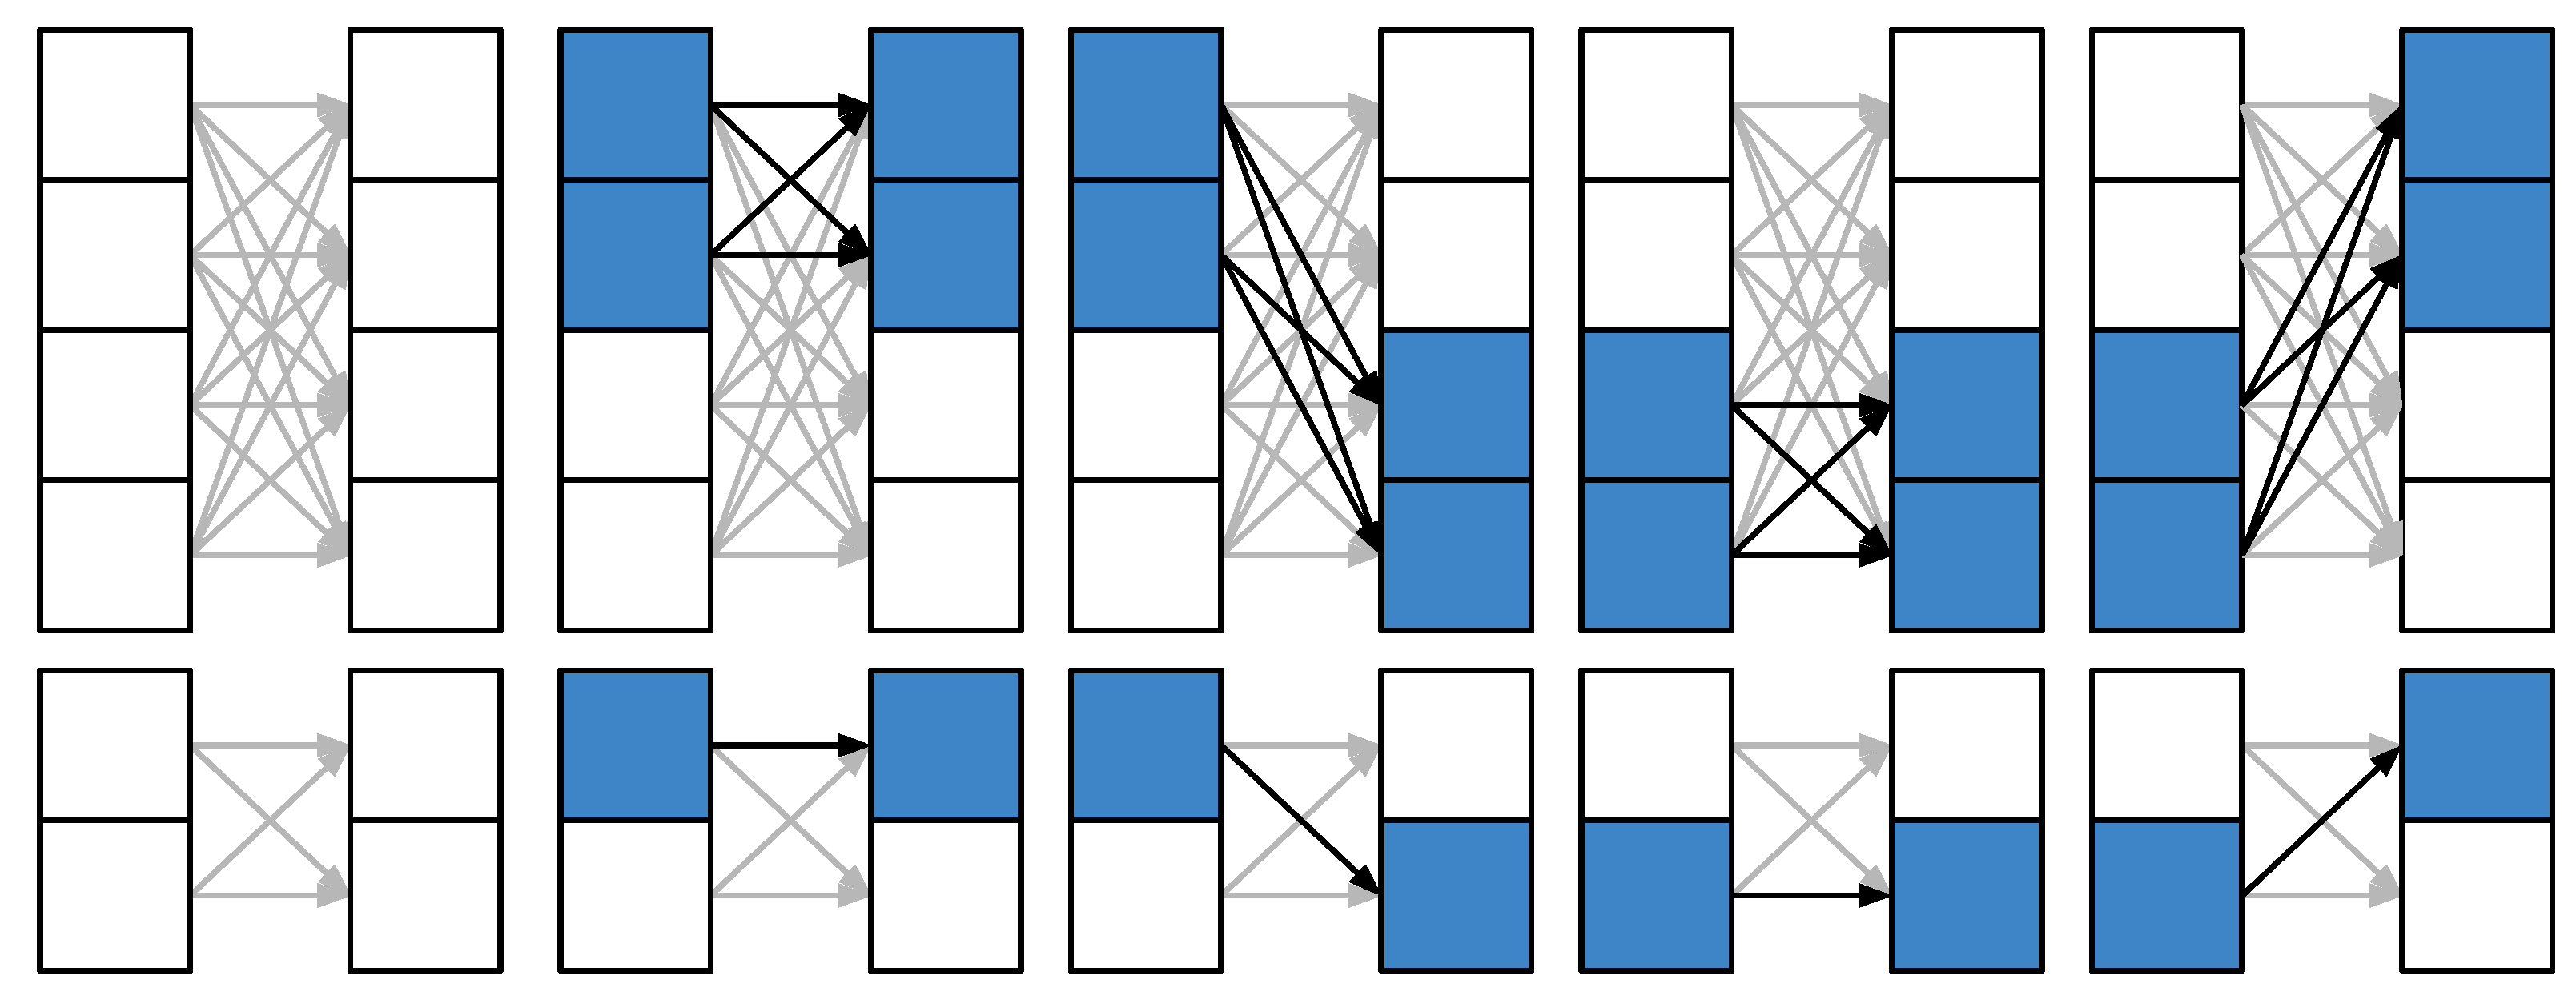
\includegraphics[width=0.8\linewidth]{fig/serialexec}
    \end{center}
    \caption{The recursive computation done by sub--layer primitive.
      Two levels of recursion are shown, each requiring less cache. }
    \label{fig:full-exec}
  \end{figure}

  This primitive is designed to efficiently use higher levels of cache
  when available, by ensuring that the order of {\bf full image
    primitives} are executed in a cache--friendly way.  This is
  achieved in a recursive fashion, where each successive recursive
  step requires half the memory of the previous step to fit the whole
  working set inside the cache.  Two levels of recursion are shown for
  the case of $\alpha = \beta = 4$ is shown on
  Fig.~\ref{fig:full-exec}.  In the first step (first row in
  Fig.~\ref{fig:full-exec}), both the number of input and output
  images are divided in half.  The next recursive step (second row in
  Fig.~\ref{fig:full-exec}) is then applied for all 4 possible
  subdivisions.  Note how the second level of recursion requires
  storage for 2 input and 2 output images in order to fit the whole
  working set inside cache, while the first level requires twice as
  much.  The order in which the 4 recursive problems are solved
  further increases cache reuse.  In the case when $\alpha \ge 2\beta$
  or $\beta \ge 2\alpha$ a simpler recursive step is performed, by
  dividing only the input/output images in half and solving two
  recursive sub--problems.

  {\bf Full layer primitive} \quad Our last primitive divides the
  computation of $B$ sets of $\alpha' S$ output images into sets of
  sub--layer primitives.  Each of $T$ available threads is statically
  scheduled to execute one or more such primitives.

  The main goal of the primitive is to equally divide the work among
  the $T$ threads such that once invoked they all finish roughly at
  the same time.  As described above, the $B$ sets of $\alpha'S$
  output images of size $D \times H \times W$ can regarded as a $5D$
  tensor of size $B \times (\alpha'S) \times D \times H \times W$.
  Again, we take a recursive approach to our static scheduling
  algorithm.  The input to our algorithm is a set of $T$ threads, and
  a $5D$ tensor of values that has to be computed.

  For the base case of our algorithm, when $T=1$, the values of the
  $5D$ tensor is scheduled on the given core to be executed by $B$
  sub--layer primitives described above.

  Our algorithm has two different recursive steps.  The first version
  of the recursive step first finds the smallest prime $p$ that
  divides $T$.  It then divides the set of $T$ threads into $p$ sets
  of $T/p$ threads, and the $5D$ tensor into $p$ equal sub--tensors by
  slicing it along the highest significant dimension that has a size
  of at least $p$.  It then recursively solves the $p$ problems for
  each set of $T/p$ threads and each equally sized sub--tensor.  If no
  dimension of the tensor is larger or equal than $p$, we apply the
  base case on an arbitrary available thread.  If the dimension of the
  tensor along which the splicing was performed is not divisible by
  $p$, another recursive problem is solved for all $T$ threads and the
  remaining sub--tensor.  Note that the size of the sub--tensor of
  each recursive sub--problem has at least $p$ times less elements.
  The rationale behind this step is that we will have each set of
  $T/p$ threads solving problems of exactly the same size.  As we
  expect them to be done roughly at the same time, when they can all
  work on computing the remaining values.

  As our previous primitives assume computation of multiple of $S$
  images, splicing along the second most significant dimension (of
  size $\alpha'S$) is done only when $\alpha' \ge p$.

  Note that in the recursive call for the remaining of the tensor, the
  value of $T$ doesn't decrease.  Thus, depth of recursion can reach
  up to $\log_2 E$, where $E$ is the number of elements in the $5D$
  tensor, which can be very large.  As the scheduling is done during
  compile--time, this can significantly increase the compile time, and
  create ``code bloat'', as primitives of many different sizes might
  have to be compiled.

  To prevent this we introduce the second version of the recursive
  step, which is applied when the number of elements of the $5D$
  tensor is smaller than $\epsilon$ times the number of elements of
  the original tensor.  In this case we divide the tensor along the
  most significant dimension larger than $T$ into $T$ sub--tensors,
  some of which are larger than others, after which $T$ base cases are
  applied and the work is scheduled on the $T$ threads.  The basic
  idea is that once computation required for the sub--tensor is small
  compared to the overall computation required for the layer, we can
  allow for some cores to do a bit more work than others without
  hurting overall performances.  In our implementation we picked
  $\epsilon$ to be $0.008$, which limits the recursion to maximal
  depth of $7$ while not allowing any single core to perform more then
  $1\%$ more work than other cores.

  \begin{figure}
    \begin{center}
      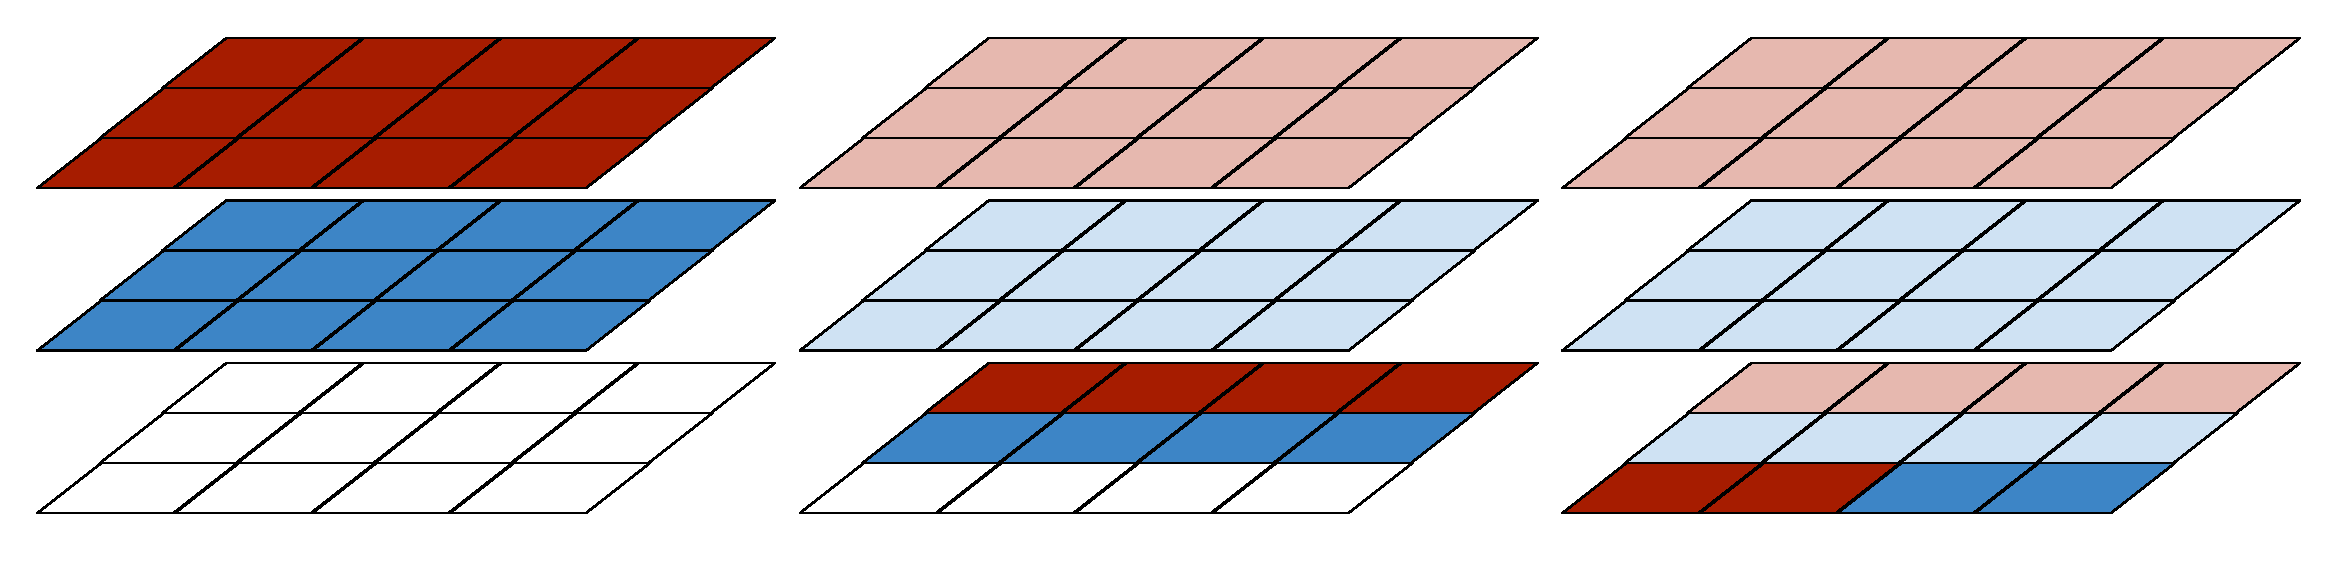
\includegraphics[width=0.97\linewidth]{fig/static2}
    \end{center}
    \caption{Computing the values of $F'=3$ channels of 2D images of
      size $4 \times 3$ using $T=2$ threads.  The three columns
      represent three stages.  The dark blue/red represent the values
      scheduled to be computed by $1^{st}/2^{nd}$ core.}
    \label{fig:problem-subdivision}
  \end{figure}

  An example of such scheduling for the special case of $B=1$, $F'=3$
  and $S=1$ and 2D images of size $4 \times 3$ is shown on
  Fig.~\ref{fig:problem-subdivision}.

  There are multiple benefits of our approach.  First, note that all
  the cores perform exactly the same computation.  When using multiple
  virtual threads per physical core, each thread can benefit from $L1$
  instruction cache.  Additionally, when multiple threads compute
  different images of the layer (as in the first step in
  Fig.~\ref{fig:problem-subdivision}), they access the elements of the
  input images in exactly the same order.  This will yield high hit
  rate of the higher levels of cache shared between cores.

  \subsection{Input image padding}

  As mentioned before, in order to be usable for the backward pass,
  our primitive has to support either implicit or explicit zero
  padding of input images.  When the input images are large, and
  kernels small, explicit zero padding of the input image only
  slightly increases the computational cost.  However, as the images
  get smaller this overhead can become significant.

  Additionally, once might consider a hybrid approach, where along
  some directions the input is explicitly padded, while along the
  other we perform implicit computation.

  We support implicit padding along an arbitrary of dimensions by
  modifying the lines 8--10 of
  Algorithm~\ref{alg:serial-forward-subtask}.  Instead of looping over
  all possible kernel offsets, for each invocation of the primitive,
  we provide additional runtime parameters, a pre--computed limits,
  for which the kernels offset are valid.
